\documentclass[12pt]{article}
\usepackage{graphicx}

\begin{document}

\section*{Apa itu Oracle APEX}
\paragraph{} Oracle APEX adalah platform Low-code yang berguna untuk membuat suatu aplikasi dengan aman dengan standar fitur kelas dunia yang bisa digunakan di mana saja


\section{Mengelola data dalam spreadsheet itu sulit}
kekurangan spreadsheet :

\begin{itemize}
	\item validasi data manual
	\item keamanandata tidak efektif
	\item untuk berbagi data sulit untuk di bagikan serta lamban
	
\end{itemize}


\section{Aplikasi yang cocok untuk Oracle APEX}

adapun jenis-jenis aplikasi yang cocok untuk Oracle APEX adalah :
\begin{itemize}
	\item Aplikasi sekala besar untuk ribuan pengguna
	\item memperbagus proses bisnis yang sudah ketinggalan jaman
	\item Aplikasi swalayan untuk semua karyawan
	\item Bukti dari konsep
	\item mengganti spreadsheet
	
\end{itemize}

\section{cara membuat workspace Oracle APEX}

\begin{itemize}
	\item Ketik link ”https://apex.oracle.com/en/” dibrowser masing masing
	\item klik ”Get started for free”
	\item klik ”Request a Free Workspace” \\	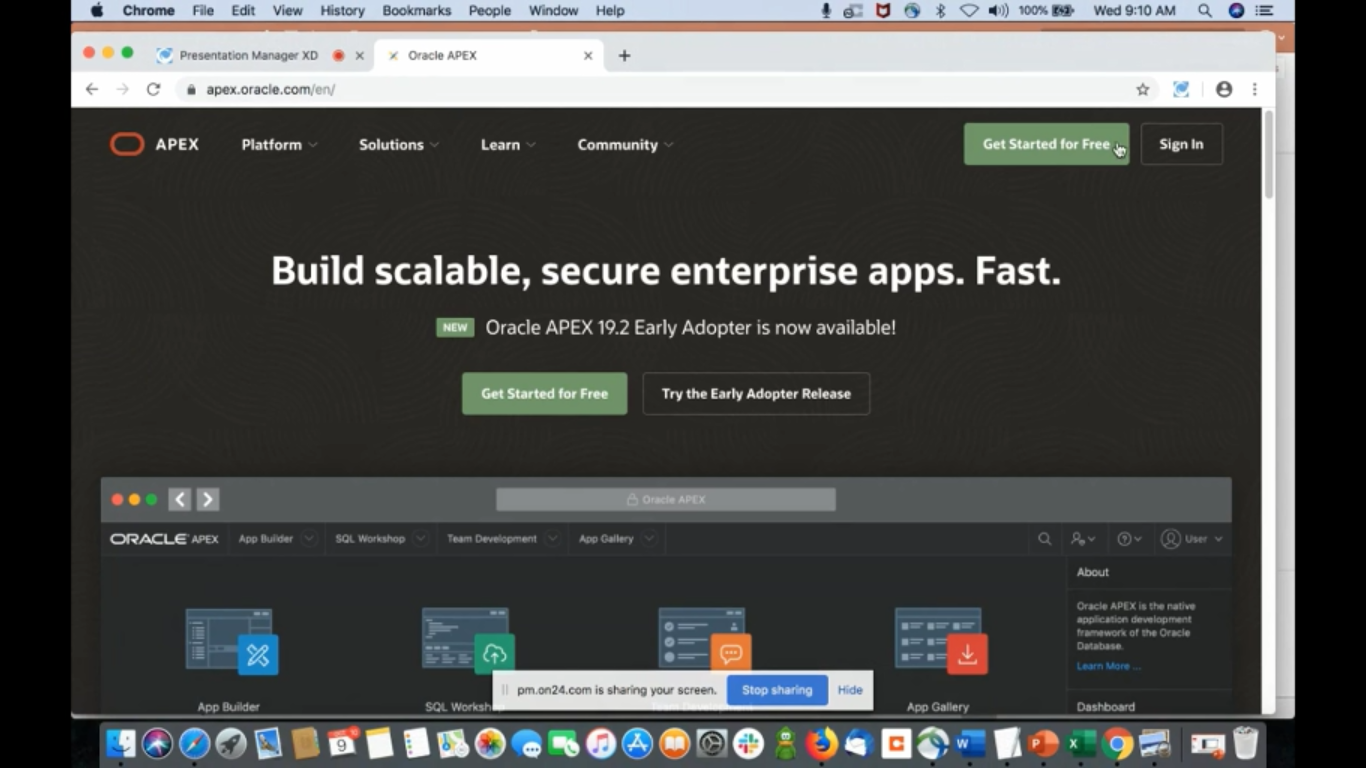
\includegraphics[scale=0.3]{pic/1}
	\item Isi form sesuai dengan yang dibutuhkan, lalu klik next\\	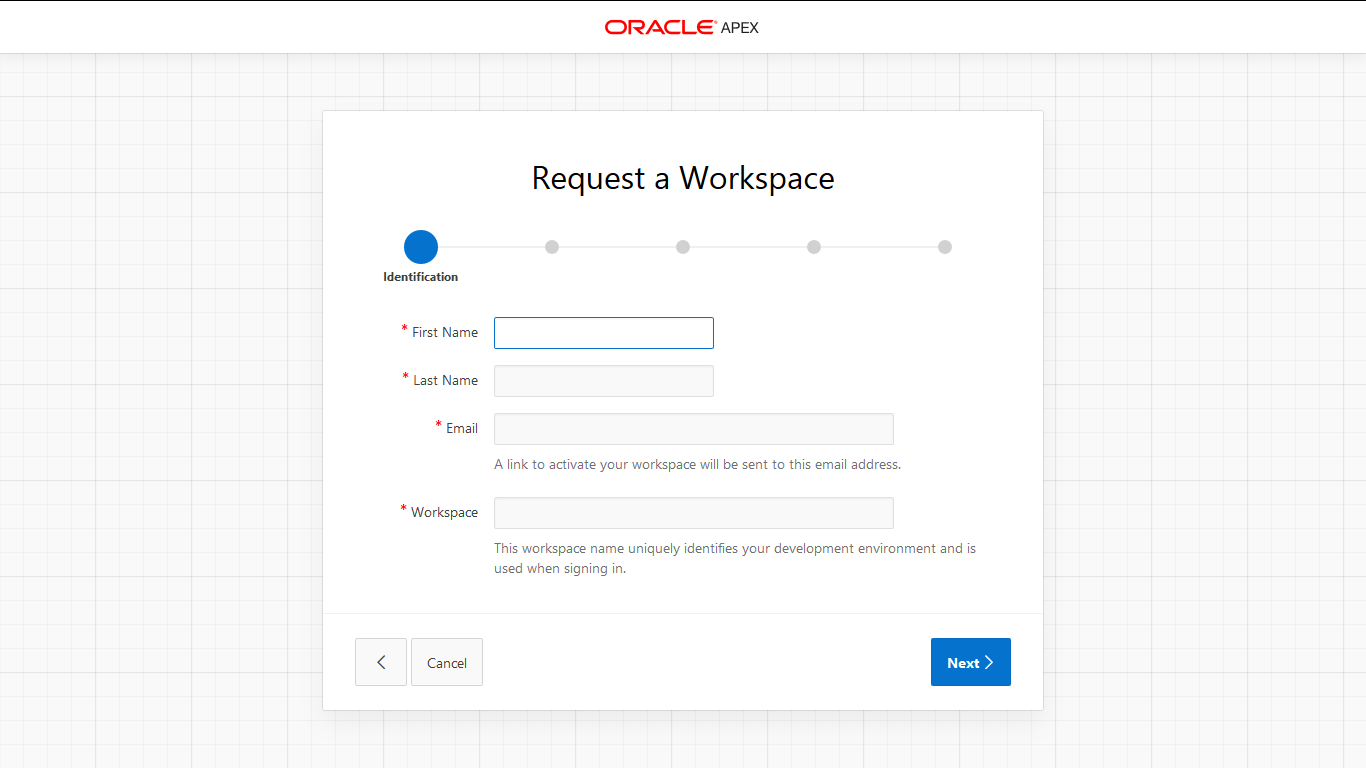
\includegraphics[scale=0.3]{pic/2}\\
	
	\item jika selesai cek email yang di gunakan untuk create wok space	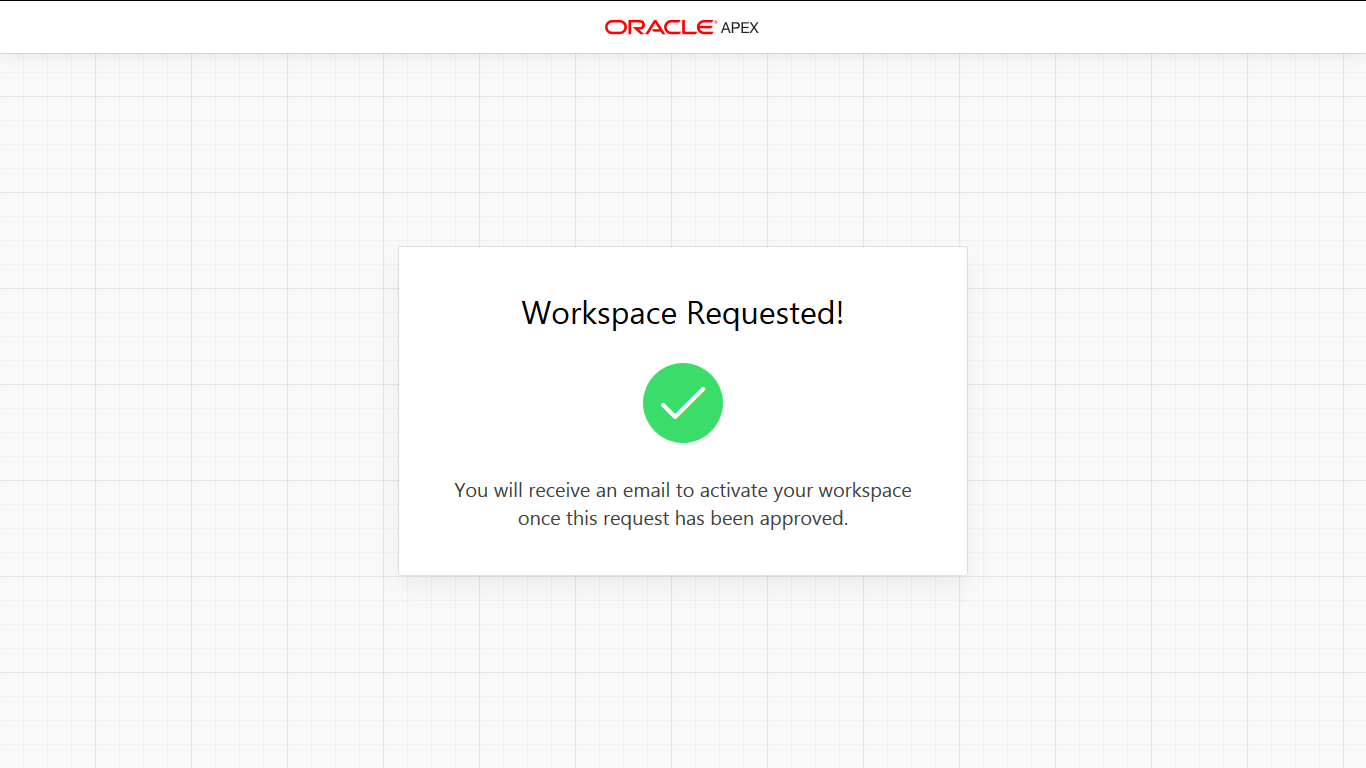
\includegraphics[scale=0.3]{pic/3}

	\item buka email dari oracle lalu klik create workspace\\
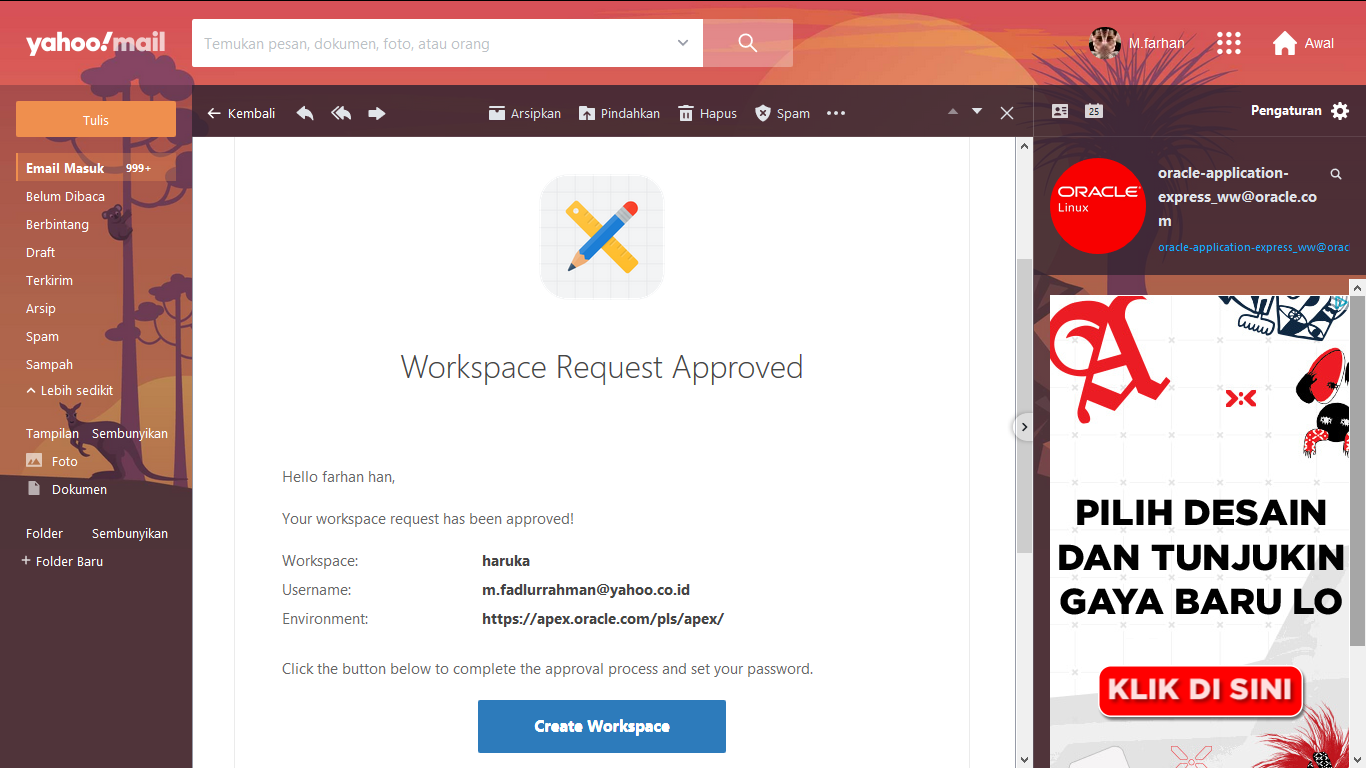
\includegraphics[scale=0.3]{pic/4}	
	
	\item lalu login ke Oracle APEX, dengan data yang sudah didaftarkan\\
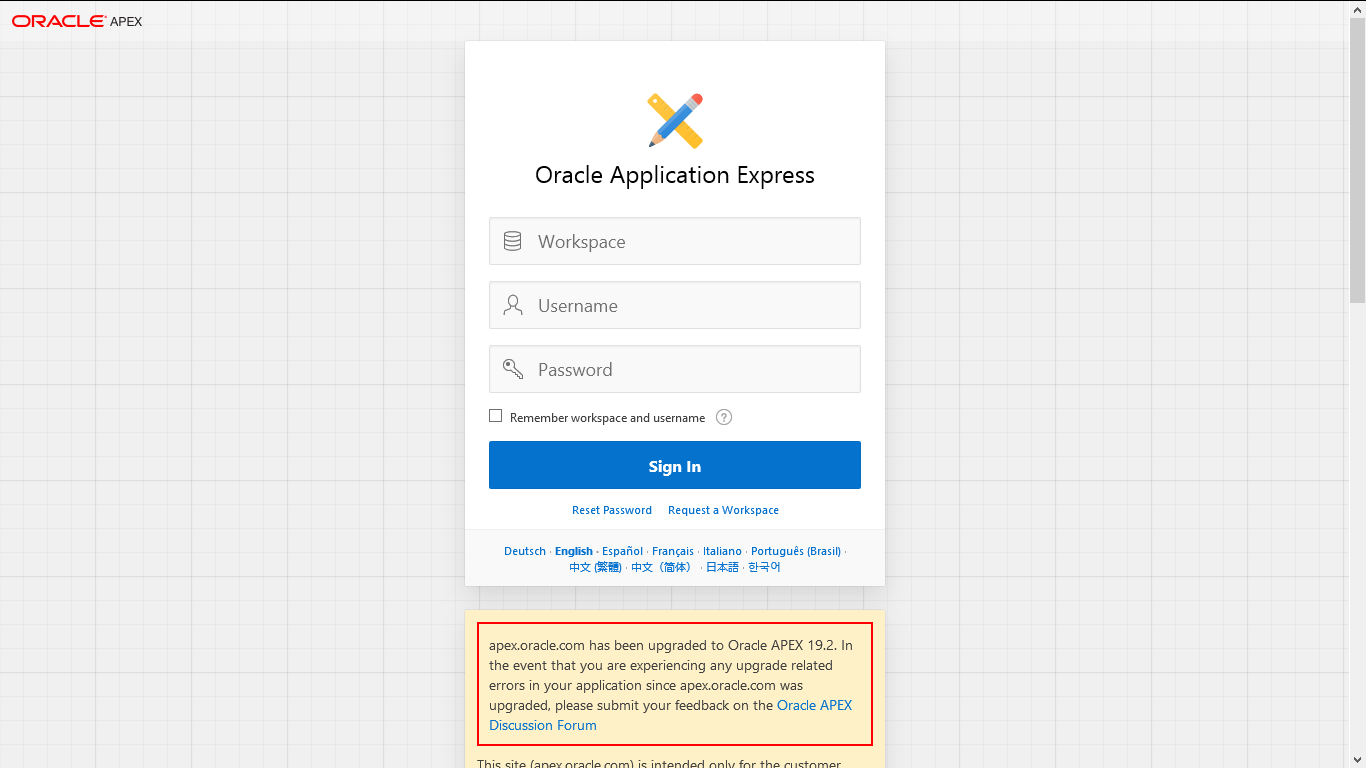
\includegraphics[scale=0.3]{pic/5}	
	
	\item tampilan sesudah login, selesai\\	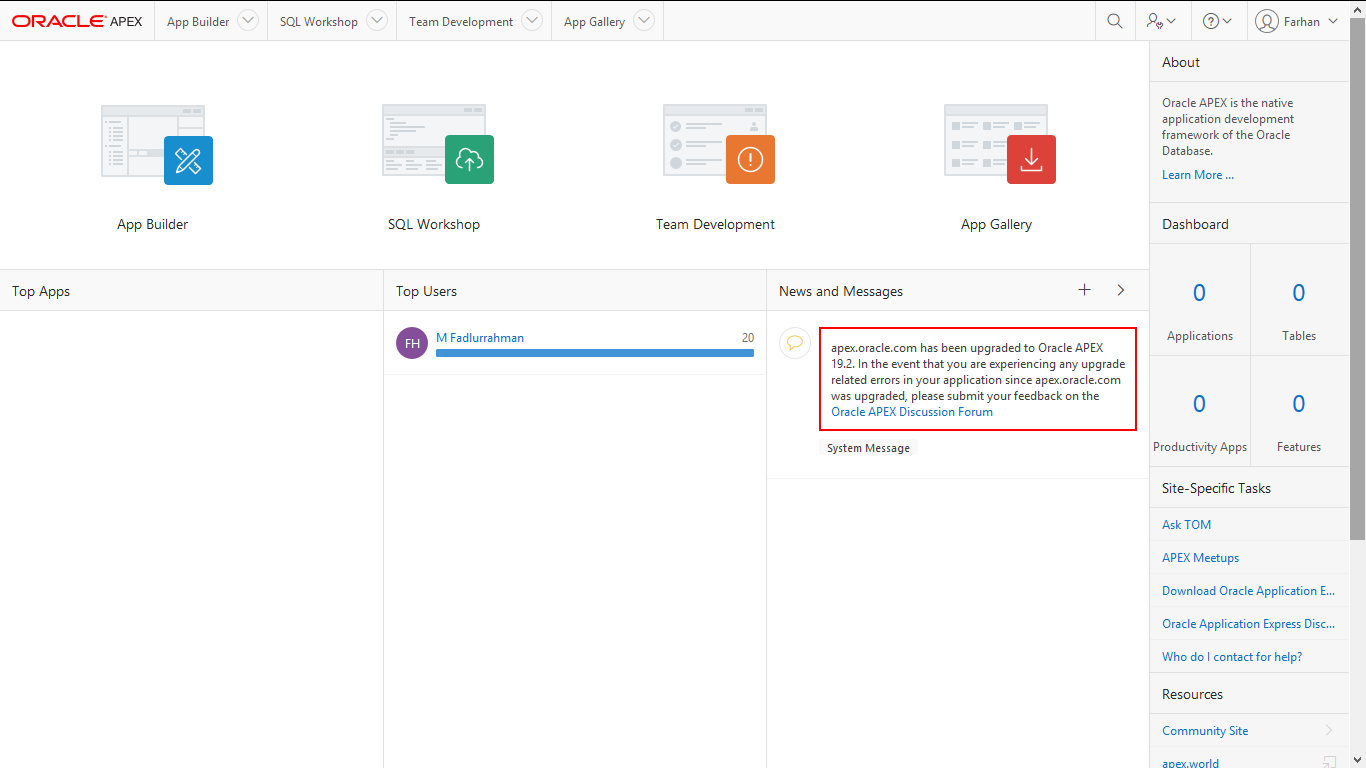
\includegraphics[scale=0.3]{pic/6}
	
\end{itemize}


\end{document}
\end{document}